% !TEX root = ../arxiv.tex
\section{Few-Shot Attribute Learning Toy Problem}
\label{app:toy_problem}

In this section, we present a toy problem that illustrates the challenges introduced by the FSAL setting and the failures of existing approaches on this task. This simple problem
captures the core elements of our FSAL tasks, including ambiguity, introducing novel attributes at test time, and the role of learning good representations. The primary limitation of this
model is the fact that it is fully linear and the attribute values are independent---in a more
realistic FSAL task recovering a good representation from the data is significantly more
challenging, and the data points will have a more complex relationship with the attributes as in our
benchmark datasets.

\paragraph{Problem setup} We define a FSAL problem where the data points $\bx
\in \bbR^{m}$ are generated from binary attribute strings, $\bz \in \{0, 1\}^d$, with $\bx = A \bz +
\bzeta$ for some matrix $A \in \bbR^{m \times d}$ with full column rank and noise source $\bzeta$.
Thus, each data point $\bx$ is a sum of columns of $A$ with some additive noise.

In each episode, examples are labelled as positive when two designated entries of the attribute strings are both 1-valued,
and negative otherwise. For the training episodes, the labels depend only on the first $d_1 < d$
entries of $\bz$. At test time, the labels depend on the remaining $d -d_1$ attributes. The training and test
episodes are generated by choosing two of the attributes in the respective sets. Then $k$ data points are sampled with positive labels (the two attributes are 1-valued) and $k$ with negative labels (at least one of the attributes is
0-valued).

\begin{figure}
    \iflatexml
        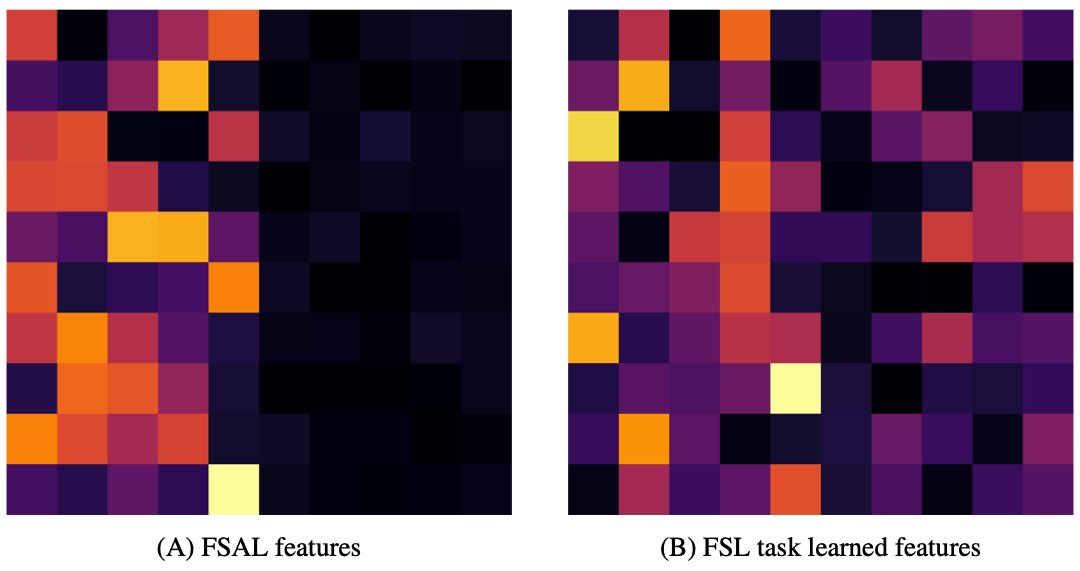
\includegraphics[width=6\linewidth]{figures/WA_abs_inferno.png}
    \else
    \begin{minipage}{0.48\linewidth}
    \centering
    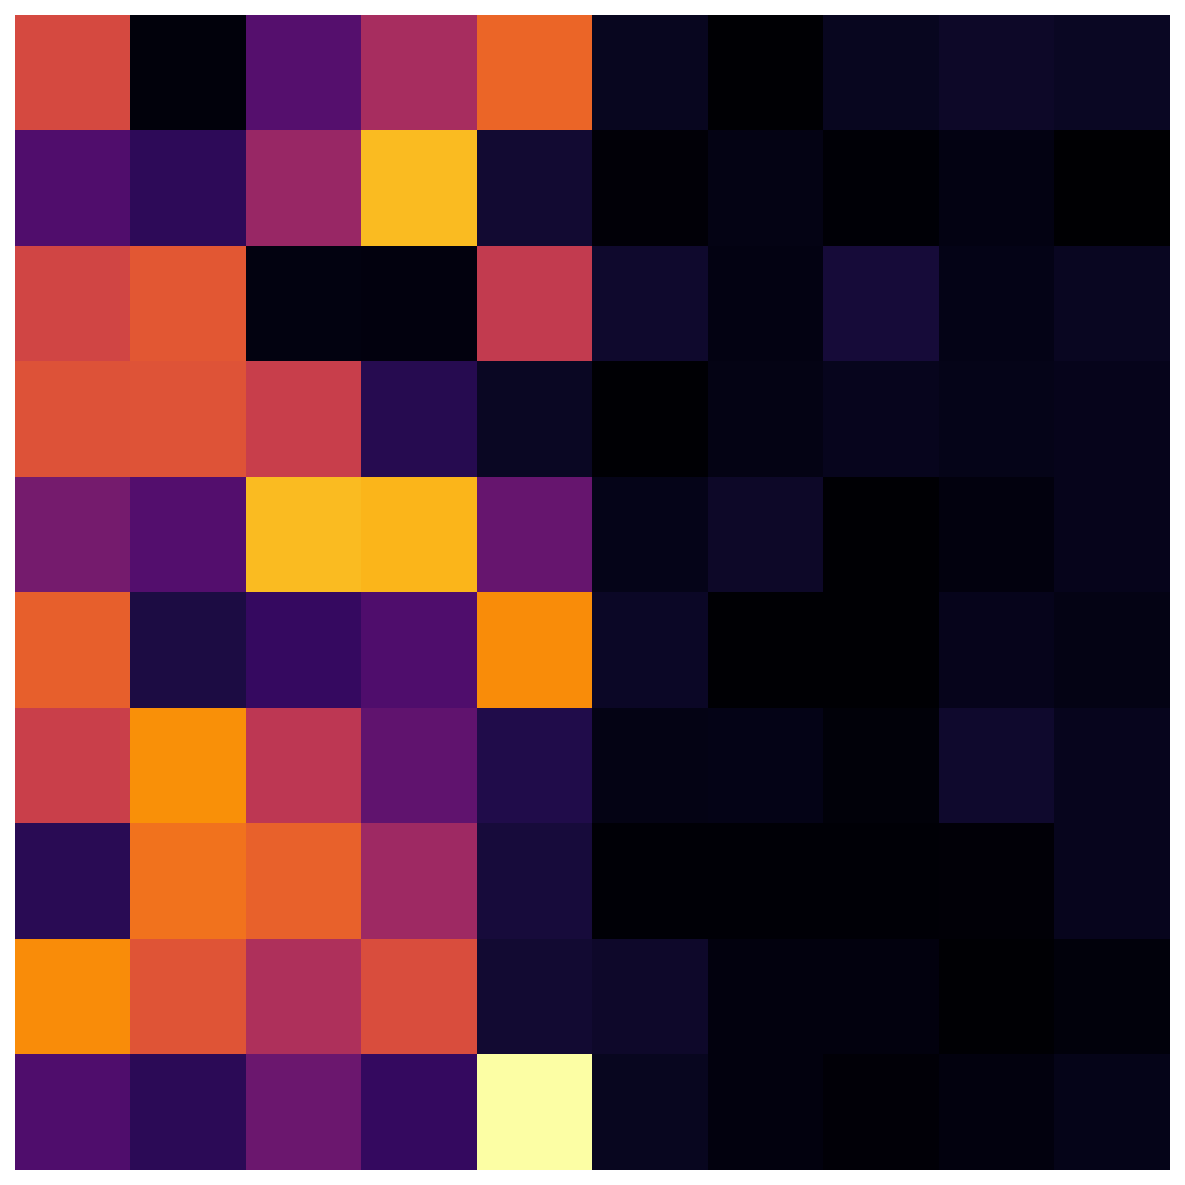
\includegraphics[width=\linewidth]{figures/WA_abs_flexible_inferno.pdf}\\
    (A) FSAL features
    \end{minipage}\hfill%
    \begin{minipage}{0.48\linewidth}
    \centering
    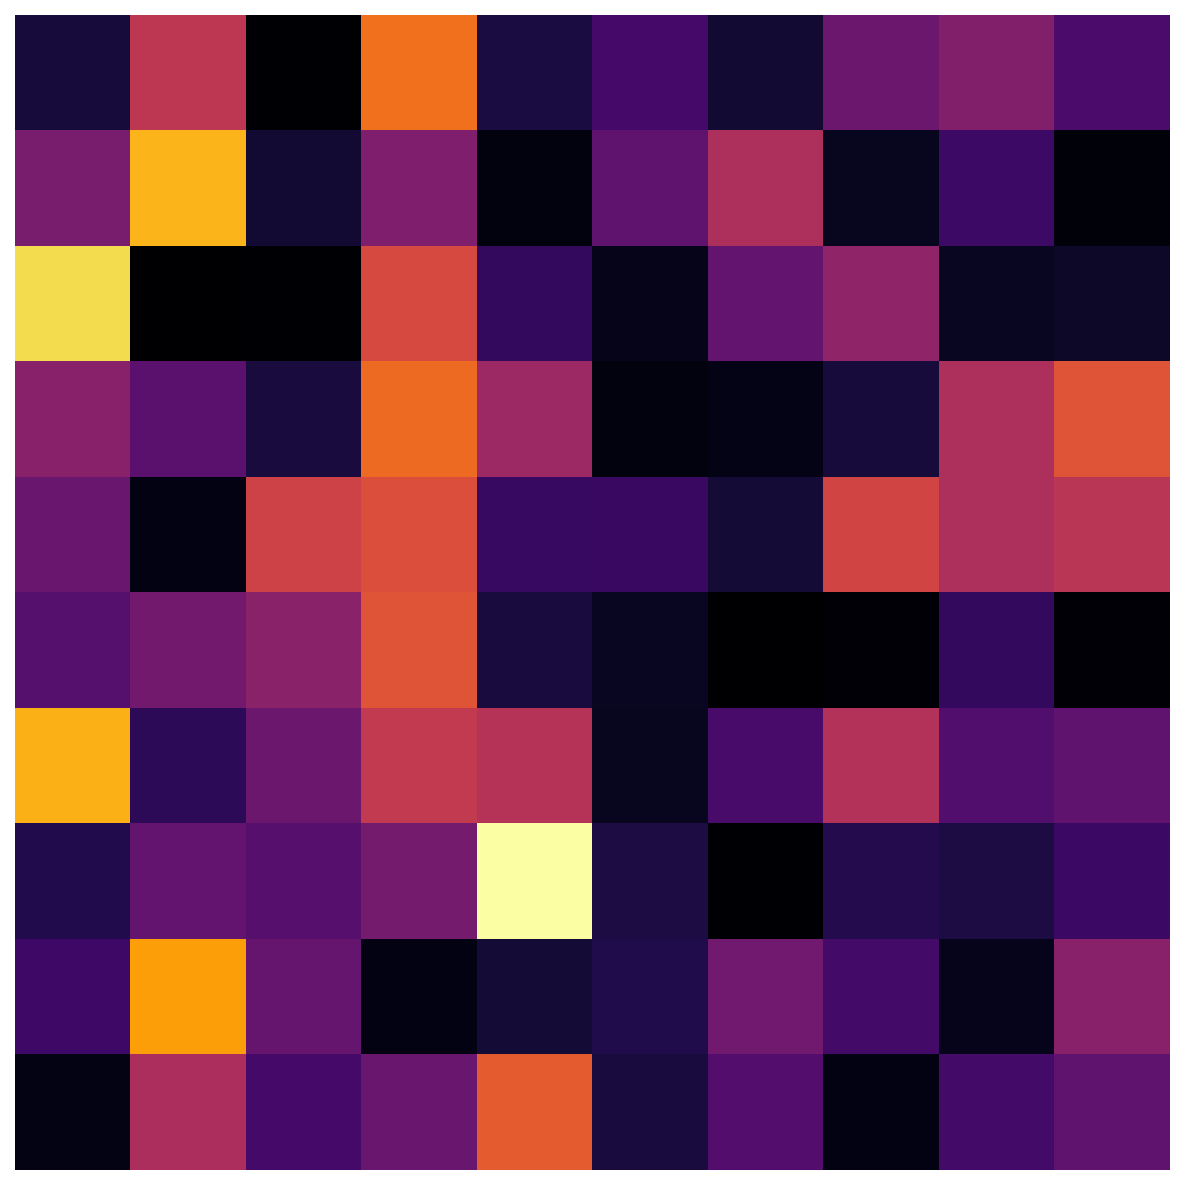
\includegraphics[width=\linewidth]{figures/WA_abs_standard_inferno.pdf}\\
    (B) FSL task learned features
    \end{minipage}
    \fi
    \caption{Projecting data features into prototypical network embedding space ($WA$) for the
    linear toy problem. Values closer to zero are darker in colour. On the FSAL task, the model
    destroys information from the test attributes to remove ambiguity at training time.}
    \label{fig:toy_problem_weights}
\end{figure}
\paragraph{Linear prototypical network} Now, consider training a prototypical network on this data
with a linear embedding network, $g(\bx)~=~W\bx$. Within each episode, the prototypical network
computes the prototypes for the positive and negative examples,
\[
\bc_{j} = \frac{1}{k}\sum_{\bx_i \in S_j} g(\bx_i)
= \frac{1}{k}\sum_{\bx_i \in S_j} \sum_{l=1}^{d}z_{il}W\ba_{l},\textrm{ for }j \in \{0, 1\},
\]
where $S_j$ is the set of data points in the episode with label $j$, and $\ba_{l}$ is the
$l^{\text{th}}$ column of the matrix $A$. Further, the prototypical network likelihood is given
by,
\[p(y=0|\bx) = \frac{\exp\left\{-\Vert W\bx - \bc_0 \Vert^2_2\right\}}{\exp\left\{-\Vert W\bx -
\bc_0 \Vert^2_2\right\} + \exp\left\{-\Vert W\bx - \bc_1 \Vert^2_2\right\}}.\] The goal of the
prototypical network is thus to learn weights $W$ that lead to small distances between data points
in the same class and large distances otherwise. In the FSAL tasks, there is
an additional challenge in that class boundaries shift between episodes. The context (the choice of attribute entries) defining the
boundary is unknown and must be inferred from the episode. However, with few shots (small $k$) there
is ambiguity in the correct context --- with a high probability that several possible contexts
provide valid explanations for the observed data.

\paragraph{Fitting the prototypical network}
Notice that under our generative model, with $\bx = W\bz + \bzeta$ and for $j \in \{0, 1\}$ we have,
\begin{align*}
W\bx - \bc_j =\ & W A (\bz - \frac{1}{k}\sum_{\bz_i \in S_j} \bz_i) + %\\ &
\frac{1}{k}\sum_{i}W\bzeta_i +
W\bzeta.
\end{align*}
% \]
Notice that if $\rvv_j(\bz) = A (\bz - \frac{1}{k}\sum_{\bz_i \in S_j} \bz_i)~\in~\textrm{Ker}(W)$,
the kernel of $W$, then the entire first term is zero. Further, if $\bz \in S_j$ (the same class as
the prototype) then there is no contribution from the positive attribute features in this term.
Otherwise, this term is guaranteed to have some contribution from the positive attribute features.

Therefore, if $W$ projects to the linear space spanned by the positive attribute features then
$W\rvv_j(\bz)$ is zero when $\bz \in S_j$ and non-zero otherwise. This means that the model will be
able to solve the episode without contextual ambiguity. Then the optimal weights are those that
project to the set of features used in the training set---destroying all information about the test
attributes which would otherwise introduce ambiguity.

We observed this effect empirically in Figure~\ref{fig:toy_problem_weights}, where we have plotted
the matrix $\mathrm{abs}(WA)$. Each column of these plots represents a column of $A$ mapped to the
prototypical network's embedding space. The first 5 columns correspond to attributes used at
training time, and the remaining 5 to those used at test time.

In the FSAL task described above, as our analysis suggests, the learned prototypical feature
weights project out the features used at test time (the last 5 columns). As a result, the model
achieved 100\% training accuracy but only 51\% test accuracy (chance is 50\%).

We also compared against an equivalent problem set up that resembles the standard few-shot learning setting. In the FSL problem, the binary attribute strings may have only a single non-zero entry and each episode is a binary classification problem where the learner must distinguish between two classes. Now the vector $\bz$ is a one-hot encoding and the comparison to the prototypes occurs only over a single feature column of $A$, thus there is no benefit to projecting out the test features. As expected, the model we learned (Figure~\ref{fig:toy_problem_weights} B) is not forced to throw away test-time information and achieves 100\% training accuracy and 99\% test accuracy.

\paragraph{Settings for Figure~\ref{fig:toy_problem_weights}} We use 10 attributes, 5 of which are
used for training and 5 for testing. We use a uniformly random sampled $A\in\bbR^{30\times10}$ and
the prototypical network learns $W\in\bbR^{10\times30}$. We use additive Gaussian noise when
sampling data points with a standard deviation of 0.1. The models are trained with the Adam
optimizer using default settings over a total of 30000 random episodes, and evaluated on an
additional 1000 test episodes. We used $k=20$ to produce these plots, but found that the result was
consistent over different shot counts.
